

\tikzset{every picture/.style={line width=0.75pt}} %set default line width to 0.75pt        

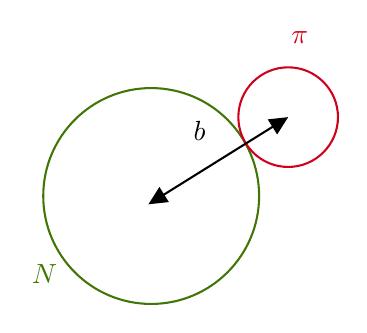
\begin{tikzpicture}[x=0.75pt,y=0.75pt,yscale=-1,xscale=1]
%uncomment if require: \path (0,300); %set diagram left start at 0, and has height of 300

%Shape: Circle [id:dp5217046923283729] 
\draw  [color={rgb, 255:red, 65; green, 117; blue, 5 }  ,draw opacity=1 ] (177,163) .. controls (177,134.28) and (200.28,111) .. (229,111) .. controls (257.72,111) and (281,134.28) .. (281,163) .. controls (281,191.72) and (257.72,215) .. (229,215) .. controls (200.28,215) and (177,191.72) .. (177,163) -- cycle ;
%Shape: Circle [id:dp22288734190325] 
\draw  [color={rgb, 255:red, 208; green, 2; blue, 27 }  ,draw opacity=1 ] (271,125) .. controls (271,111.75) and (281.75,101) .. (295,101) .. controls (308.25,101) and (319,111.75) .. (319,125) .. controls (319,138.25) and (308.25,149) .. (295,149) .. controls (281.75,149) and (271,138.25) .. (271,125) -- cycle ;
%Straight Lines [id:da9107173582949104] 
\draw    (230.21,165.41) -- (292.45,126.59) ;
\draw [shift={(295,125)}, rotate = 148.05] [fill={rgb, 255:red, 0; green, 0; blue, 0 }  ][line width=0.08]  [draw opacity=0] (8.93,-4.29) -- (0,0) -- (8.93,4.29) -- cycle    ;
\draw [shift={(227.67,167)}, rotate = 328.05] [fill={rgb, 255:red, 0; green, 0; blue, 0 }  ][line width=0.08]  [draw opacity=0] (8.93,-4.29) -- (0,0) -- (8.93,4.29) -- cycle    ;

% Text Node
\draw (170,194.4) node [anchor=north west][inner sep=0.75pt]  [color={rgb, 255:red, 65; green, 117; blue, 5 }  ,opacity=1 ]  {$N$};
% Text Node
\draw (295,82.4) node [anchor=north west][inner sep=0.75pt]  [color={rgb, 255:red, 208; green, 2; blue, 27 }  ,opacity=1 ]  {$\pi$};
% Text Node
\draw (248,125.4) node [anchor=north west][inner sep=0.75pt]  [color={rgb, 255:red, 0; green, 0; blue, 0 }  ,opacity=1 ]  {$b$};


\end{tikzpicture}